\section{React Native}
\label{sec:Frameorks_ReactNative}

Das von Meta entwickelte React Native Framework ermöglicht die Cross-Plattform Entwicklung mit JavaScript.
Als Zielplattformen werden neben Android und iOS unter anderem Windows und macOS unterstützt \cite{ReactNative}.
Ein großer Vorteil des Frameworks ist die Verwendung der in der Web-Entwicklung verbreiteten \ac{UI}-Bibliothek React.
Für Webentwickler fällt die Einarbeitung in React Native leicht, was zu einer großen Verbreitung des Frameworks führt \cite{Appfigures_TopSDKs,Stackoverflow_2022}.
Außerdem lässt sich React Native vergleichsweise einfach in bestehende native Projekte integrieren.
Diese Integrationsmöglichkeit führt auch dazu, dass neben den Apps von Meta, weitere populäre Apps wie die Microsoft Office Apps, Pinterest und WordPress Teile ihrer Funktionalität mit React Native umsetzen \cite{ReactNative_Showcase}.


Obwohl React Native wie Cordova und Capacitor JavaScript verwendet, wählt das Framework einen anderen Ansatz, um die Cross-Plattform Entwicklung zu ermöglichen.
Mit Ionic können Cordova und Capacitor Apps ebenfalls React als \ac{UI}-Bibliothek verwenden.
Dabei ist die Oberfläche komplett als Webanwendung implementiert und wird in einer WebView dargestellt.
ReactNative nutzt stattdessen die nativen \ac{UI}-Komponenten der jeweiligen Plattformen.
Durch die Kombination von Webtechnologien und nativer \ac{UI} ist React Native als Haybrid Bridged App zu betrachten.

%TODO: eventuell nur eine der Architekturen vorstellen -> besprechen

Aktuell wird die Architektur von React Native grundlegend angepasst, um Probleme der bisherigen Architektur zu lösen.
Da dieser Prozess noch nicht abgeschlossen ist, wird hier sowohl auf die bisherige als auch auf die neue Architektur eingegangen.

Die bisherige Architektur setzt sich aus zwei Komponenten zusammen, welche über die sogenannte React Native Bridge miteinander kommunizieren.
Die Bridge trennt dabei den JavaScript-Code von der nativen Umgebung.
Der JavaScript-Code wird innerhalb der Ausführungsumgebung JavaScriptCore, einem Teil der Open-Source Browser Engine WebKit, ausgeführt.
JavaScriptCore läuft in einem eigenen Thread, der auch als JavaScript-Thread oder kurz JS-Thread bezeichnet wird.
Unter iOS ist die WebKit Engine Teil des Betriebssystems und kann von allen React Native-Apps genutzt werden.
Android stellt JavaScriptCore nicht bereit, weshalb React Native-Apps für Android JavaScriptCore mitliefern müssen und demnach größer ausfallen \cite{Dragomir_ReactNative,Nawrocki_Comparison_Hybrid_Native_Frameworks}.
Die Business-Logik der App wird in JavaScript implementiert und im JS-Thread ausgeführt.
Die \ac{UI} wird von der nativen Umgebung, dem sogenannten nativen Thread, gerendert.
Jegliche Kommunikation zwischen den beiden Threads erfolgt über die Bridge, wie in \autoref{fig:reactnative_bridge} schematisch dargestellt.
Die Kommunikation zwischen den Threads erfolgt über Nachrichten im \ac{JSON} Format \cite{ReactNative_newArchitecture,Dragomir_ReactNative}.
Render-Anweisungen werden vom JS-Thread an den nativen Thread gesendet und umgekehrt werden Eingaben und Events an den JS-Thread übermittelt.
Zusätzlich können im nativen Thread sogenannte Native Modules ausgeführt werden, die es erlauben beliebigen nativen Code zu verwenden \cite{ReactNative_TurboModules}.
\begin{figure}[ht]
  \centering
  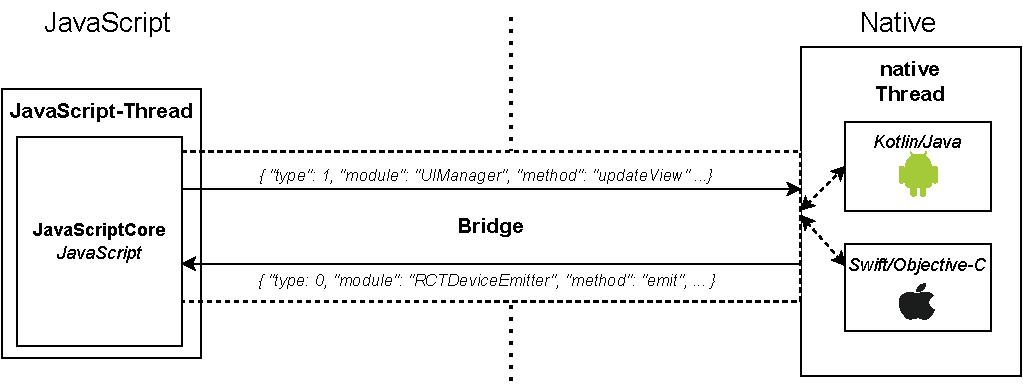
\includegraphics[width=0.85\textwidth]{reactnative_bridge.pdf}
  \caption{Austausch von JSON-Nachrichten zwischen JS-Thread und nativem Thread über die  React Native Bridge.}
  \label{fig:reactnative_bridge}
\end{figure}

Aufgrund des hohen Overheads durch die Kommunikation über \ac{JSON}-Nachrichten, kann es zu Performance-Problemen beim Rendern der \ac{UI} kommen, wenn viele Nachrichten ausgetauscht werden müssen.
Zum Beispiel beim Scrollen von Listen oder bei Animationen werden viele Nachrichten zwischen den beiden Threads ausgetauscht.
In der Folge werden neue Listen-Elemente verzögert gerendert und Animationen erreichen durch den Kommunikationsoverhead keine ausreichende Framerate damit sie flüssig wirken \cite{Cook_ReactNativeBridge}.

\begin{figure}[ht]
  \centering
  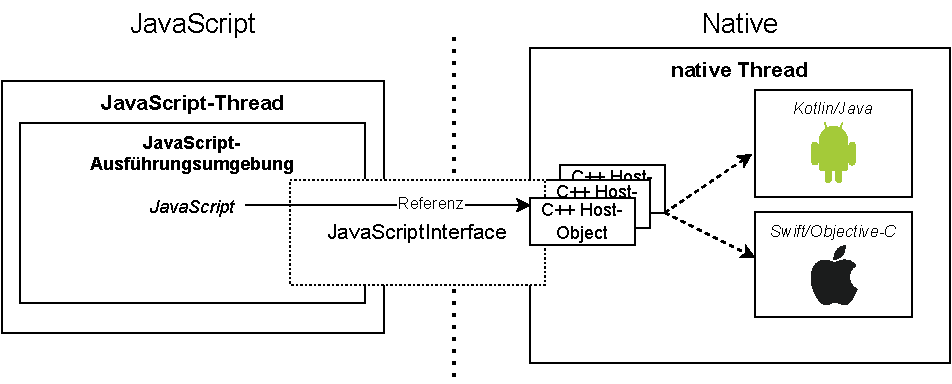
\includegraphics[width=0.85\textwidth]{reactnative_newArchitecture.pdf}
  \caption{Neue Architektur von React Native. Zugriff von JavaScript auf native Host-Objects über das \ac{JSI}.}
  \label{fig:reactnative_newArchitecture}
\end{figure}
Die neue Architektur, dargestellt in \autoref{fig:reactnative_newArchitecture}, soll unter anderem diese Probleme lösen und synchrone Kommunikation zwischen den beiden Threads ermöglichen.
Zur Kommunikation wird die React Native Bridge durch eine neue Schnittstelle das sogenannte \ac{JSI} ersetzt \cite{Cook_ReactNativeBridge}.
Die neue Schnittstelle erlaubt es, in JavaScript-Code Referenzen auf C++-Objekte, sogenannte Host-Objects zu verwenden.
Methoden dieser Objekte können aus JavaScript heraus aufgerufen werden und können beliebigen C++-Code ausführen oder auch auf Objekte der nativen Sprachen der Plattform zugreifen \cite{Parashuram_React}.

Die Kommunikation kommt ohne Serialisierung aus, was in vielen Fällen zu Verbesserungen der Performance führt.
Zum Beispiel beim Anwendungsfall einer Kamerasteuerung, wie in \autoref{fig:reactnative_nativeModules} gezeigt, kann die Aufnahme-Funktion eine Referenz auf ein Bild zurückgeben, anstatt das Bild zu serialisieren und über die Bridge zu übertragen.
Auf dieser Referenz können weitere Funktionen zum Beispiel zur Bearbeitung, aufgerufen werden \cite{Parashuram_React}.
\begin{figure}[ht]
  \centering
  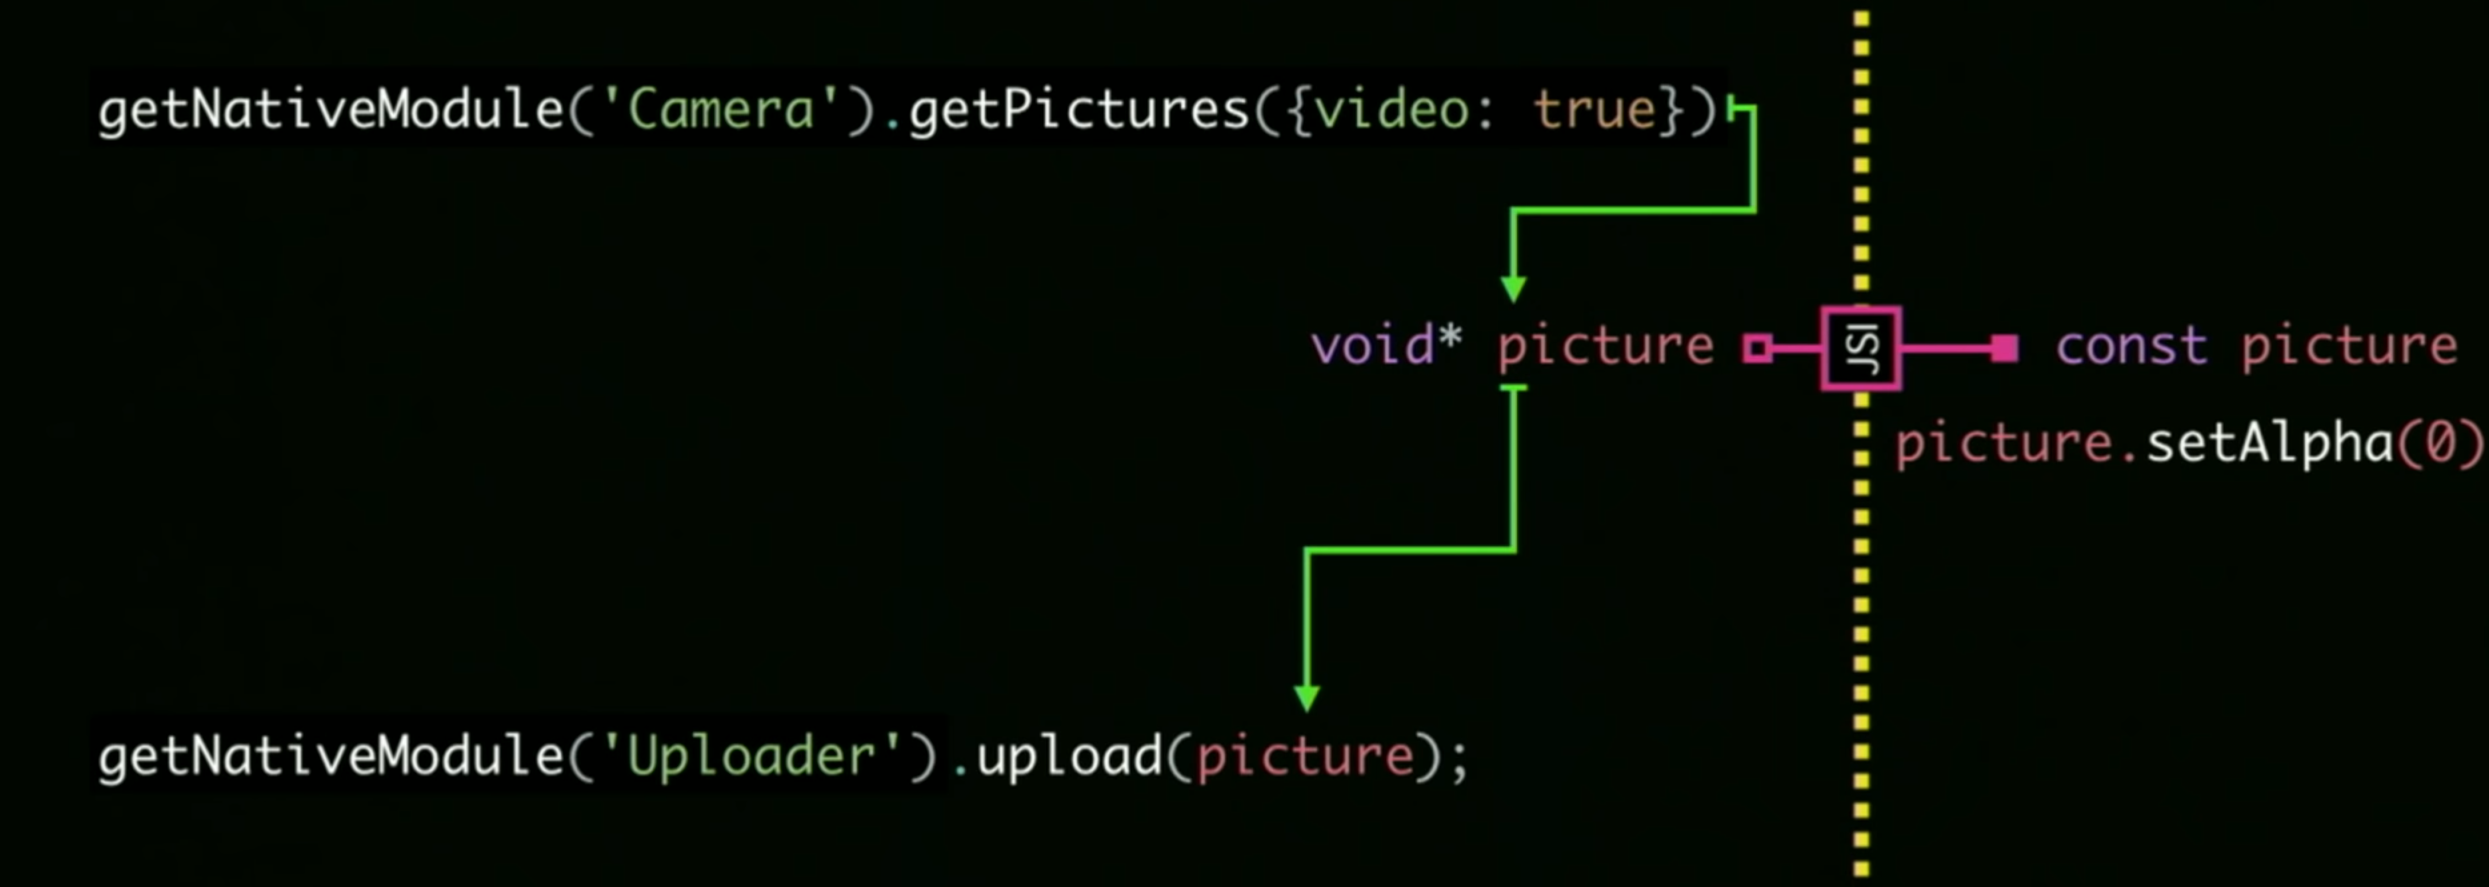
\includegraphics[width=0.75\textwidth]{reactnative_nativemodules}
  \caption{Vorteile der neuen Architektur für den Zugriff auf native Funktionen \cite{Parashuram_React}.}
  \label{fig:reactnative_nativeModules}  
\end{figure}
Der Aufruf von nativem Code bei React Native ähnelt durch die neue Architektur auch dem Aufruf von \ac{DOM}-Funktionen durch JavaScript im Browser.
\ac{DOM}-Funktionen werden beispielsweise genutzt, um Elemente einer Webseite zu manipulieren.
Dazu greift JavaScript auf Funktionen eines vom Browser bereitgestellten Objekts zu, welche wiederum die zugrundeliegenden Funktionen im nativen Code des Browsers aufrufen \cite{ReactNative_newArchitecture}.
Parashuram \cite{Parashuram_React} bezeichnet den Aufruf von nativer Funktionalität auch als \ac{RPC} zwischen JavaScript und nativem Code.

Die neue Architektur vereinfacht darüber hinaus das Ersetzen der JavaScript Ausführungsumgebung.
Bisher war aufgrund engen Kopplung der Ausführungsumgebung und der Bridge nur JavaScriptCore möglich.
Über einfache Adapter lassen sich neben JavaScriptCore beispielsweise auch die leichtgewichtige, für React Native optimierte Hermes Engine oder Googles V8 Engine verwenden \cite{Cook_ReactNativeBridge,JSI_Adapter}.

Wie in der alten Architektur kann auch in der neuen Architektur beliebiger nativer Code im nativen Thread ausgeführt werden.
Dazu kommt eine neue Variante der Native Modules, die sogenannten Turbo Native Modules, zum Einsatz \cite{ReactNative_TurboModules}.
Diese verwenden ebenfalls Host-Objects um C++-Funktionen in JavaScript verfügbar zu machen, welche wiederum nativen Code aufrufen können \cite{Parashuram_React}.


Durch die Verwendung von nativen \ac{UI}-Elementen ist die Performance von React Native bei \ac{UI}-Operationen vergleichbar mit nativen Apps und besser als bei hybriden Apps mit Cordova oder Capacitor \cite{Huber_UI}.
Ähnlich wie Xamarin unter iOS, fallen React Native Apps unter Android durch die Mitlieferung der JavaScript-Engine vergleichsweise groß aus \cite{Nawrocki_Comparison_Hybrid_Native_Frameworks}.
Durch die neue Architektur und die einfachere Integration anderer JavaScript-Engines, kann dieses Problem in Zukunft vermutlich durch die Verwendung der vom Betriebssystem bereitgestellten Engine gelöst werden.
Die Performance von React Native ist sehr stark vom Anwendungsfall abhängig.
Beispielsweise sind \ac{CPU} intensive Berechnungen deutlich langsamer als bei nativen Apps, während \ac{I/O} Aufgaben, wie zum Beispiel Web-Requests ähnlich schnell sind \cite{Nawrocki_Comparison_Hybrid_Native_Frameworks}.
Beim Zugriff auf native Funktionen schneidet React Native besser ab als Flutter, Cordova und Capacitor.
Vergleichswerte zu Xamarin fehlen hier jedoch \cite{Biorn-Hansen_PerformanceOverhead_CrossPlatform}.

In der Stackoverflow-Umfrage 2022 \cite{Stackoverflow_2022} geben von allen Entwicklern, welche bereits mit React Native gearbeitet haben, eine Mehrheit von knapp 56 \% an, dass sie das Framework auch weiterhin einsetzen wollen.
Damit schneidet React Native besser ab als Xamarin und Cordova, aber schlechter als Capacitor und Flutter.
Bei Betrachtung der Entwickler, ohne Erfahrung mit dem Framework, welche interessiert daran sind es einzusetzen, liegt React Native jedoch nur knapp hinter dem auch in dieser Kategorie beliebtesten Framework Flutter.